\section{\whoscoredplain\ crawler}

There are several steps one must go through in order to populate the database in \cref{sec:database-overview}. For each season, one must first gather the IDs for all the matches. When the IDs are gathered, one can start traversing all matches, gathering scorelines, event information, player statistics, etc. Below comes a description of how to locate the different data sources, and how to extract the data.


\subsection{URL structure}

When crawling \whoscored\  for data, one must know where the web pages containing the wanted data are located. Every match, team, and player listed on \\ \whoscored\ has its own unique ID, given as an integer number. Regions, leagues, seasons, and season stages also has their own unique IDs. Different entity types have their own URL structure. The only difference between the URLs of two entities of the same kind are their IDs.


\subsection{Match IDs}

Season fixtures are available at the following URLs:

\whoscoredurl{/Regions/REGION/Tournaments/TOURNAMENT/Seasons/SEASON/Stages/STAGE/Fixtures},

where \textbf{REGION} is the region of the tournament, \textbf{TOURNAMENT} the tournament in question, \textbf{SEASON} the season to fetch fixtures for, and \textbf{STAGE} the stage of the season. For league tournaments, the stage ID stays the same. For knockout tournaments, there are different stages per season (qualification, group stage, and knockout stage). The example below points to the fixture list for the English Premier League 2016-2017:

\whoscoredurl{/Regions/252/Tournaments/2/Seasons/6335/Stages/13796/Fixtures},

where 252 is the region ID for England, 2 the tournament ID for the English Premier League, 6335 the season ID for the English Premier League 2016-2017, and 13796 the stage ID for the season.

Fixtures are grouped by year and month. Finished matches are marked with the final score, while coming matches are marked with "\textbf{vs}". The matches are listed in a large table, with one row for each match, as shown in \cref{fig:whoscored-fixture-list}.

\begin{figure}
    \centering
    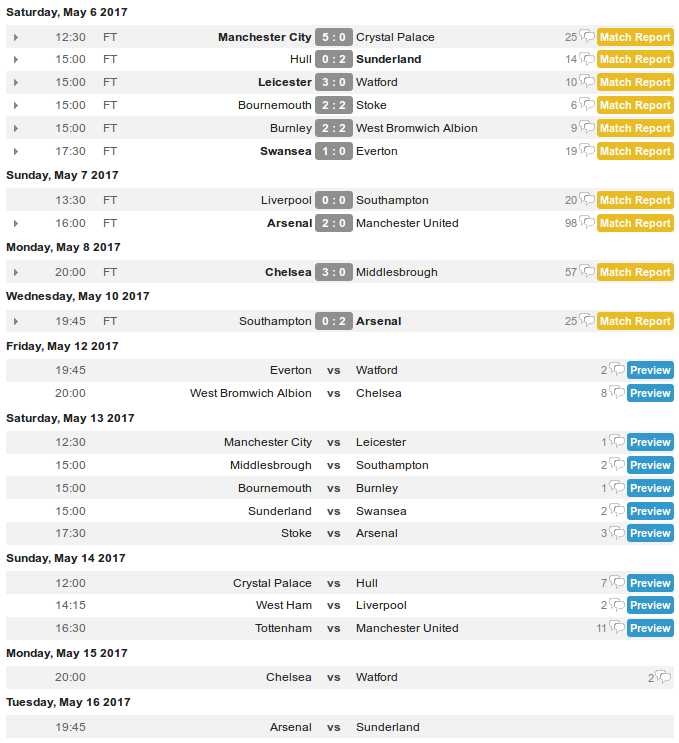
\includegraphics[width=0.9\textwidth]{whoscored/fixture-list.png}
    \caption{Small portion of the match fixtures for English Premier League, May 2017.}
    \label{fig:whoscored-fixture-list}
\end{figure}

The row elements contain the ID for each match. Extracting the match ID is as simple as fetching the \url{data-id} attribute from the row element. The example below shows the row element for Arsenal versus Manchester United May 7, 2017.
\begin{lstlisting}[language=HTML,caption={Hypertext to Arsenal versus Manchester United May 7, 2017.}]
<tr class="item" data-id="1080862">...</td>
\end{lstlisting}


\subsection{Match data}

Match URLs are of the following form:

\whoscoredurl{/Matches/ID/VIEW},

where \textbf{ID} is the match ID, and \textbf{VIEW} is the view. A match has several views, depending on whether it is detailed or not, and whether it is finished, ongoing or not started. The different views are listed in \cref{tab:whoscored-match-views}. The example below points to the \url{Live} view showing detailed match event information for Arsenal versus Manchester United May 7, 2017.

\whoscoredurl{/Matches/1080862/Live}

\subsubsection{Match events}

Match event data is located at the \url{Live} match view. Event data is stored in three different locations, depending on detail level. All match event data is located in JavaScript variables in the source code of the respective web page. Fetching the data can easily be done using simple regular expressions.

The minimum match details are located in a variable called \textit{matchHeader}. A description of the data in the match header is shown in \cref{tab:whoscored-match-header-data}. The example below is from Arsenal versus Manchester United May 7, 2017.
\begin{lstlisting}[language=JavaScript,caption={Match header from Arsenal versus Manchester United May 7, 2017.}]
matchHeader.load([13,32,'Arsenal','Manchester United','07/05/2017 16:00:00','07/05/2017 00:00:00',6,'FT','0 : 0','2 : 0',,,'2 : 0','England','England']);
\end{lstlisting}
13 and 32 are the team IDs of Arsenal and Manchester United, respectively. The match started at "07/05/2017 16:00:00". The status code 6 indicates that the match is complete. FT indicates that the match was ended at full time. No goals were scored during the first half. Arsenal won the match 2-0. Both teams are located in England.

Extracting the match header from the web page source code can be done using the following regular expression:
\begin{lstlisting}[language=Python,caption={Regular expression used to extract match header data.}]
    /matchHeader\.load\((.+?)\);/
\end{lstlisting}

The intermediate match details are located in a variable called \textit{initialMatchDataForScrappers} \textit{[sic]}. The variable contains the match header, lineups, substitutions and most important match events. Extracting the intermediate match details from the web page source code can be done using the following regular expression:
\begin{lstlisting}[language=Python,caption={Regular expression used to extract initialMatchDataForScrappers.}]
    /var initialMatchDataForScrappers = (.+?);/
\end{lstlisting}

The full match details are located in a variable called \textit{matchCentreData}. The variable is divided into three main parts: general information, home team information, and away team information. The included information is described in \cref{subsec:whoscored-match-details}. Extracting the full match details from the web page source code can be done using the following regular expression:
\begin{lstlisting}[language=Python,caption={Regular expression used to extract matchCentreData.}]
    /var matchCentreData = (.+?);/
\end{lstlisting}


\subsubsection{Head to head information}

Head to head information is located at the \url{Show} match view.

Previous meetings (up to six matches) between the two teams are listed in a table, with one row for each match, as shown in \cref{fig:whoscored-previous-meetings}. For each match, there is a hypertext to the match web page.
\begin{figure}
    \centering
    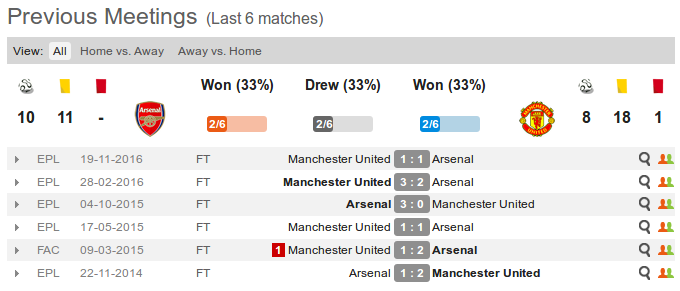
\includegraphics[width=\textwidth]{whoscored/previous-meetings.png}
    \caption{Previous meetings between Arsenal and Manchester United before the match May 7, 2017.}
    \label{fig:whoscored-previous-meetings}
\end{figure}

The example below is from Arsenal versus Manchester United May 7, 2017, showing a hypertext to their last meeting.
\begin{lstlisting}[language=HTML,caption={Hypertext to the last meeting before the match between Arsenal and Manchester United May 7, 2017.}]
    <a class="..." href="/Matches/1080633/Live/England-Premier-League-2016-2017-Manchester-United-Arsenal">1 : 1</a>
\end{lstlisting}
One can extract the match ID from the hypertext using the following regular expression on the hypertext URL:
\begin{lstlisting}[language=Python,caption={Regular expression used to extract match ID from hypertext.}]
    /Matches/(\d+)/
\end{lstlisting}

Previous matches (also up to six matches) for the two teams are listed in the same way.

Team characteristics for the two teams are listed as three different sets of characteristics: strengths, weaknesses, and styles. All characteristics are given a textual description. Strengths and weaknesses are also given indications of their levels (very weak, weak, strong, very strong).
\begin{figure}
    \centering
    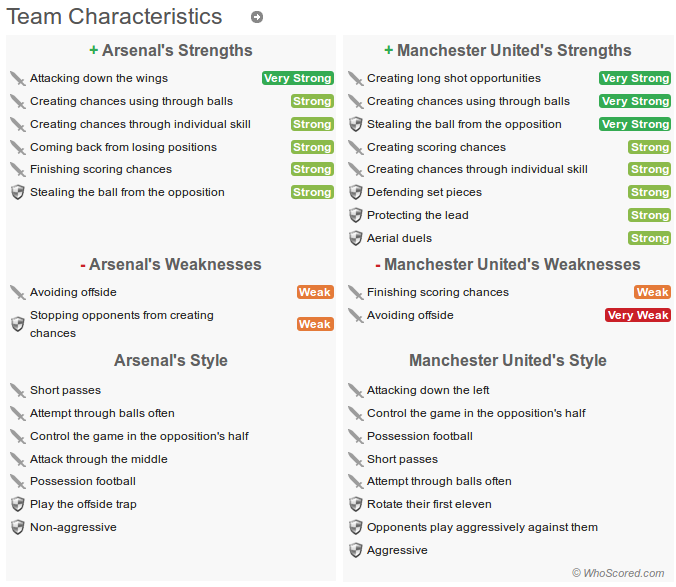
\includegraphics[width=\textwidth]{whoscored/team-characteristics.png}
    \caption{Team characteristics for Arsenal and Manchester United before the match May 7, 2017.}
    \label{fig:whoscored-team-characteristics}
\end{figure}

\clearpage